Skemalægningsprogrammet Docendo er et brugervenligt samt forholdsvis simpelt program. Programmet  danner en kalender med uger og dage, hvorefter brugeren har mulighed for at justere diverse parametre alt efter behov. Heriblandt tager programmet bland andet højde for, at nogle skoler har forskellige fag, og giver derfor brugeren mulighed for at tilføje flere fag. Samtidig har brugeren mulighed for at tilpasse lektionernes længde, hvilket giver programmet fleksibilitet. Dernæst fastlåser programmet lokaler og lærere, som har undervisning på bestemte tidspunkter. Det forhindrer dobbeltbookninger i et bestemt lokale eller lignende. Hvis et problem skulle opstå, kan lektionerne flyttes.\footfullcite{docendo}
\begin{figure}[!h]
  \centering
  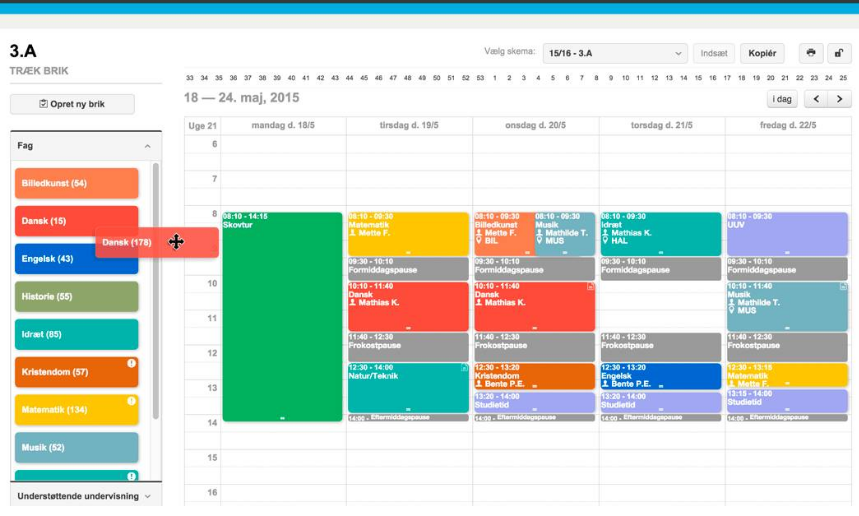
\includegraphics[width=\textwidth]{partials/graphics/docendo.png}
    \caption{Eksempel på skemplanlægning i Docendo.\footfullcite{docendob}}
  \label{fig:docendo}
\end{figure}

Da Docendo ikke genererer et endeligt skema, men et skema, som skal rettes i, betyder det at der stadig skal investeres en mængde tid i skemaplanlægningen.